\graphicspath{{5induction/asy/}}
\section{Mathematical Induction and Well-ordering}\label{chap:induction}

In Section \ref{sec:proof} we discussed three methods of proof: direct, contrapositive, and contradiction. The fourth standard method, \emph{induction,} has a very different flavor. Before giving a formal definition, we consider how the need for induction arguments often arises.

\subsection{Iterative Processes \& Proof by Induction}\label{sec:induction}

Recursive processes are very common in mathematics and its applications: an unknown $x_n$ satisfies a simple recurrence relation $x_{n+1}=f(x_n)$ where an initial value $x_1$ is given. The typical approach to such problems is to \emph{hypothesize} a general formula $x_n=g(n)$ (spot a pattern!), and then \emph{prove} the validity of the formula. Induction is the proof method often employed in such situations. To get us started, we investigate a famous game.


\boldsubsubsection{The Tower of Hanoi}

Circular disks of decreasing radius are stacked on three pegs. Disks are moved one at a time from the top of a stack onto an empty peg or on top of a larger disk. If we start with 10 disks on the first peg, how many moves are required to transfer all disks to another peg?\smallbreak

To get a feel for the problem, try playing the game with smaller numbers of disks. Suppose $n$ disks require $r_n$ moves. Then:
\begin{itemize}\itemsep0pt
  \item $r_1=1$ since there is only one disk to move!
  \item $r_2=3$ as shown in the picture.
\end{itemize} 

\begin{center}
	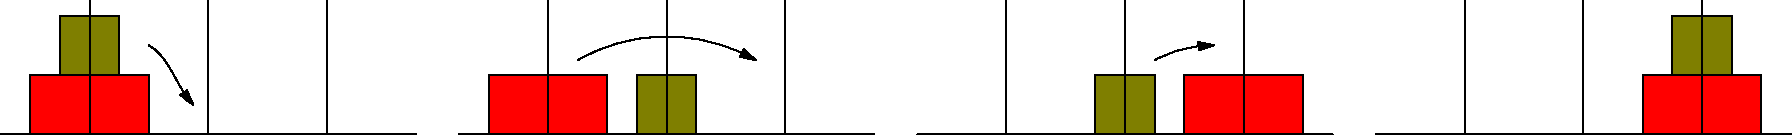
\includegraphics[width=0.9\textwidth]{induction-03-hanoi2}
\end{center}

More experimentation will hopefully convince you that $r_3=7$, at which point you might be ready to hypothesize a general formula---if not, experiment more!

\begin{conj}{}{hanoi}
	The Tower of Hanoi with $n$ disks requires $r_n=2^n-1$ moves.
\end{conj}

To make progress, consider a stack of $n+1$ disks. To move the largest disk, \emph{all other disks must be stacked on a single peg.} Moving $n+1$ disks is therefore a three-step process:
\begin{enumerate}\itemsep0pt
  \item Move the smallest $n$ disks to another peg.
  \item Move the largest disk.
  \item Move the remaining disks on top of the largest.
\end{enumerate}
\begin{center}
\href{http://www.math.uci.edu/~ndonalds/math13/induction-01-hanoi.html}{
	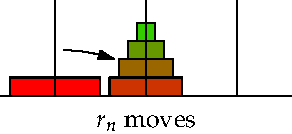
\includegraphics{induction-04-hanoirn3}\quad
	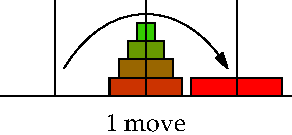
\includegraphics{induction-04-hanoirn4}\quad
	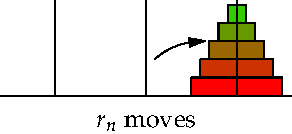
\includegraphics{induction-04-hanoirn5}
}
\end{center}


The upshot is that $r_n$ satisfies a \emph{recurrence relation}: $r_{n+1}=r_n+1+r_n=2r_n+1$.

\goodbreak

We are now in a position to prove our conjecture.

\begin{proof}
	Certainly the formula $r_n=2^n-1$ holds when $n=1$ disk (1 disk requires $r_1=1$ move).\smallbreak
	Now suppose that $n$ disks require $r_n=2^n-1$ moves, where $n\in\N$ is some fixed number. Then $n+1$ disks require
	\[
		r_{n+1}=2r_n+1=2(2^n-1)+1 =2^{n+1}-1
	\]
	moves ($\ast$). Since $n$ was arbitrary, we have in fact proved an \emph{infinite collection of implications}: 
	\[
		r_1=2^1-1\implies r_2=2^2-1\implies r_3=2^3-1 \implies \cdots \implies r_n=2^n-1\implies \cdots
	\]
	Since the first of these propositions ($r_1=2^1-1$) is true, we conclude that $r_n=2^n-1$ for all $n\in\N$.
\end{proof}

To answer the original question, 10 disk require $r_{10}=2^{10}-1=1023$ moves; at one move per second this would take 17 minutes, 3 seconds.



\boldsubsubsection{Proof by Induction}

The Tower of Hanoi argument is an example of \emph{proof by induction.} This method is invoked when we want to prove a sequence of propositions $P(1)$, $P(2)$, $P(3)$, \ldots, one for each natural number. The abstract structure of an induction proof consists of two separate arguments:
\begin{description}%\itemsep0pt
  \item[\normalfont(\emph{Base case})] Prove that $P(1)$ is true.
  \item[\normalfont(\emph{Induction step})] Prove, for each $n\in\N$, that $P(n)\Longrightarrow P(n+1)$. During this phase, $P(n)$ is termed the \emph{induction hypothesis.}
\end{description}
The result is an infinite chain of implications:
\[
	P(1)\implies P(2)\implies P(3)\implies P(4)\implies P(5)\implies \cdots
\]
Since $P(1)$ is true (base case), \emph{all} the remaining propositions $P(2)$, $P(3)$, $P(4)$, \ldots{} are also true.\smallbreak

Re-read the Tower of Hanoi proof; can you separate the base case and induction step? Our presentation was informal since we were only introducing the concept. For a formal argument, a few modifications should be made.

\begin{itemize}
  \item \emph{Set-up} the proof: orient the reader by stating, ``We prove by induction.'' It might also be helpful to spell out the propositions $P(n)$ and to tell the reader what variable ($n$) controls the induction.
  \item Label the \emph{base case} and \emph{induction step} so the reader knows what you are doing!
  \item After the induction step is complete, state your \emph{conclusion.} In the above we would replace everything after ($\ast$) with, ``By mathematical induction, $r^n=2^n-1$ for all $n\in\N$.''
\end{itemize}


Here is a straightforward and famous result, where we write the proof in our new language.

\begin{thm}{}{ind1}
	The sum of the first $n$ positive integers is $\sum\limits_{k=1}^nk=\frac 12n(n+1)$
\end{thm}

You should be familiar with summation notation $\sum\limits_{k=1}^nk=1+2+3+\cdots+n$: if not \emph{ask}!

\goodbreak



\begin{proof}
	We prove by induction. For each $n\in\N$, let $P(n)$ be the proposition $\smash{\sum\limits_{k=1}^nk=\frac 12n(n+1)}$.
	\begin{description}
		\item[\normalfont\emph{Base case} ($n=1$):] \smash{$\sum\limits_{k=1}^1k=1=\frac 121(1+1)$,} says that $P(1)$ is true.
		\item[\normalfont\emph{Induction Step}:] Fix $n\in\N$, and assume that $P(n)$ is true \emph{for this $n$.} We compute the sum of the first $n+1$ positive integers and use our induction hypothesis $P(n)$ to simplify:
	  \begin{align*}
			\sum_{k=1}^{n+1}k&=\textcolor{blue}{\sum_{k=1}^nk}+(n+1)=\textcolor{blue}{\frac 12n(n+1)}+(n+1) \tag{\textcolor{blue}{induction hypothesis}}\\
			&=\left(1+\frac 12n\right)(n+1)=\frac 12(n+2)(n+1)\\
			&=\frac 12(n+1)\bigl[(n+1)+1\bigr]
	  \end{align*}
	Therefore $P(n+1)$ is true.
	\end{description}
	By mathematical induction, we conclude that $P(n)$ is true for all $n\in\N$. That is
	\[
		\forall n\in\N,\quad \sum\limits_{k=1}^nk=\frac 12n(n+1)\tag*{\qedhere}
	\]
\end{proof}

Note how we grouped $\frac 12(n+1)\bigl[(n+1)+1\bigr]$ so that it is obviously the right hand side of $P(n+1)$.\smallbreak

We present several more examples in a similar vein, but done a little faster. As is typical, we don't explicitly introduce the symbol $P(n)$, though you should feel free to continue doing this if you find it helpful. Aim for a layout like these in your formal writing. 


\begin{example}{}{ind3}
	We prove by induction that, for all $n\in\N$,
	\[
		2+5+8+\cdots+(3n-1)=\frac 12n(3n+1) \tag{$\ast$}
	\]
	\begin{description}\itemsep0pt
		\item[\normalfont\emph{Base case} ($n=1$):] The proposition ($\ast$) is trivially true: $2=\frac 12\cdot 1\cdot(3\cdot 1+1)$.
		\item[\normalfont\emph{Induction Step}:] Fix $n\in\N$ and assume ($\ast$) holds for this value of $n$. Then
		\begin{align*}
			\textcolor{blue}{2+5+\cdots+(3n-1)}+[3(n+1)-1]&=\textcolor{blue}{\frac 12n(3n+1)}+3n+2\\
			&=\frac 12(3n^2+7n+4) =\frac 12(n+1)(3n+4)\\
			&=\frac 12(n+1)\bigl[3(n+1)+1\bigr]
		\end{align*}
		which is the required proposition for $n+1$.
	\end{description}
	By mathematical induction ($\ast$) holds for all $n\in\N$.
\end{example}

For brevity we labelled the desired proposition (what we'd have called $P(n)$) by $(\ast)$ so it could be referenced. The structure is similar to Theorem \ref{thm:ind1}: since the goal is to evaluate a sum, the induction step is little more than adding the same thing ($3n+2$) to both sides of the \textcolor{blue}{induction hypothesis}. In fact, the example could have been proved directly by invoking Theorem \ref{thm:ind1}---can you see how?
\medbreak\goodbreak

Our next two examples are a little harder, requiring more creativity to invoke the induction hypothesis. Both could alternatively be proved directly using modular arithmetic (Chapter \ref{chap:gcd}).

\begin{examples}{}{ind2}
	\exstart We prove by induction that $\forall n\in\N$, the integer $17^n-4^n$ is divisible by 13.
	\begin{enumerate}\setcounter{enumi}{1}
		\item[]\begin{description}
			\item[\normalfont\emph{Base case} ($n=1$):] Plainly $17^1-4^1$ is divisible by 13.
			\item[\normalfont\emph{Induction Step}:] Fix $n\in\N$ and assume that $17^n-4^n=13k$ for some $k\in\Z$. Then
			\begin{align*}
				17^{n+1}-4^{n+1}&=17\bigl(\textcolor{blue}{17^n}\bigr)-4^{n+1}=17\bigl(\textcolor{blue}{13k+4^n}\bigr)-4^{n+1} \tag{\textcolor{blue}{induction hypothesis}}\\
				&=17\cdot 13k+(17-4)4^n =13\bigl(17k+4^n\bigr)
			\end{align*}
			is divisible by 13.
		\end{description}
		By mathematical induction, $17^n-4^n$ is divisible by 13 for all $n\in\N$.		
		
		\item\label{ex:ind22} We prove by induction: if $n\in\N$, then $n(n+1)(2n+1)$ is divisible by 6.
		\begin{description}
			\item[\normalfont\emph{Base case} ($n=1$):] The proposition reads $1\cdot (1+1)\cdot (2\cdot 1+1)=6$, which is divisible by 6.
			\item[\normalfont\emph{Induction Step}:] Fix $n\in\N$ and assume that $\textcolor{blue}{n(n+1)(2n+1)=6k}$ for some $k\in\Z$. Then
			\begin{align*}
					(n+1)(n+2)\bigl[2(n+1)+1\bigr]-\textcolor{blue}{6k}&=\textcolor{blue}{(n+1)}\bigl[(n+2)(2n+3)-\textcolor{blue}{n(2n+1)}\bigr]\\
					&=(n+1)\bigl(2n^2+7n+6-(2n^2+n)\bigr) =6(n+1)^2
				\end{align*}
			from which
			\[
				(n+1)\bigl[(n+1)+1\bigr]\bigl[2(n+1)+1\bigr] =6\bigl((n+1)^2+k\bigr)
			\]
			is divisible by 6.
		\end{description}
		By mathematical induction, $n(n-1)(2n-1)$ is divisible by 6 for all $n\in\N$.	
	\end{enumerate}
\end{examples}


\boldinline{Scratch work is your friend!}

Unless things are very simple, you should build an induction argument by starting with some scratch work for the hard part: the \emph{induction step.} If you're stuck, explicitly stating the propositions $P(n)$ and $P(n+1)$ might help you see how to manipulate one into the other. Here are the propositions for Example \ref{ex:ind2}.1:
\begin{quote}
	\begin{tabular}{ll}
	$P(n)$: &$17^n-4^n=13k$ for some integer $k$\\[5pt]
	$P(n+1)$: &$17^{n+1}-4^{n+1}=13l$ for some integer $l$
	\end{tabular}
\end{quote}
Since $17^n$ is common to both, you could try multiplying both sides of $P(n)$ by 17; if you re-read the example, you'll see that this is essentially the induction step! For Example \ref*{ex:ind2}.2, you might try multiplying out the cubic expressions
\[
	n(n+1)(2n+1)\ \text{ and }\ (n+1)(n+2)(2n+3)
\]
and comparing coefficients. Since the leading term in both is $n^3$, the \emph{difference} is quadratic and therefore much easier to think about\ldots\smallbreak

Remember that scratch work isn't a proof; while your scratch work may make perfect sense to you, if a reader cannot follow it without assistance, then it isn't a proof! It is essential, once you think you understand the induction step, to lay out the entire proof cleanly: \emph{set-up, base case, induction step, conclusion.} As an example of what happens when you don't, here is a typical attempt at Example \ref{ex:ind3} by a student who is new to induction:

\begin{tcolorbox}[exstyle]\vspace{-10pt}
	\begin{align*}
		P(n+1)=\hspace{4pt}&2+5+\cdots+(3n-1)+[3(n+1)-1] =\smash{\frac 12}(n+1)\bigl[3(n+1)+1\bigr]\\
		&\frac 12n(3n+1)+(3n+2) =\frac 12(n+1)(3n+4)\\
		&3n^2+n+6n+4 =3n^2+7n+4
	\end{align*}
\end{tcolorbox}

Is this convincing to you? While there are many issues,\footnote{\textbullet\lstsp $P(n)$ There is no \emph{set-up, base case} or \emph{conclusion} and the word \emph{induction} is missing. The argument needs some English!
\begin{itemize}\itemsep0pt
  \item $P(n)$ has not been \emph{defined}. If you don't define it, don't write it!
  \item $P(n+1)$ is a \emph{proposition}: it cannot \emph{equal} a number! Replacing ``$P(n+1)=$'' with ``$P(n+1)\Longleftrightarrow$'' would correct this.
  \item There are no conditional connectives to indicate the logical flow. Moreover, read top to bottom, the argument is essentially $P(n)\wedge P(n+1)\implies T$, rather than the correct induction step $P(n)\implies P(n+1)$.
\end{itemize}} the student's work isn't without merit, since the required calculation is present (left side of 1\st{} line $=$ left side of 2\nd). While helpful as scratch work, a substantial re-write is needed to make this convincing.
\medbreak

We finish this section with a trickier example of this thinking at work.

\begin{example}{}{}
	An \emph{L-shaped tromino} is an arrangement of three squares in an ``L'' shape. We claim:\par
	\begin{minipage}[t]{0.75\linewidth}\vspace{-4pt}
		\begin{quote}
			If \textcolor{Magenta}{any} single square is removed from a $2^n\times 2^n$ square gird, then the remaining grid may be tiled by L-shaped trominos.
		\end{quote}
		\vspace{-6pt}
		The claim has the form $\forall n\in\N,P(n)$, but note that $P(n)$ is itself \textcolor{Magenta}{universal}. The picture shows one of the \emph{sixteen} possible examples when $n=2$. To get an idea of how to structure the induction step, think how you might use $2\times 2$ grids to analyse a $4\times 4$ grid. The picture shows how!
		\begin{itemize}
		  \item Whatever square we remove, one quarter of the $2^2\times 2^2$ grid is a $2^1\times 2^1$ grid with one square removed: this is \textcolor{blue}{tilable}.
		\end{itemize}
	\end{minipage}
	\hfill
	\begin{minipage}[t]{0.24\linewidth}\vspace{0pt}
		\flushright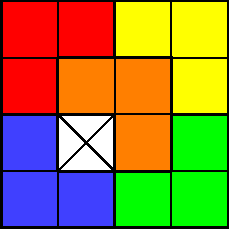
\includegraphics{induction-11-tilingexample}
	\end{minipage}
	\par
% \begin{center}
% 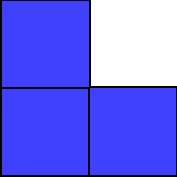
\includegraphics{induction-08-bluetromino} \qquad \qquad 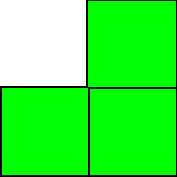
\includegraphics{induction-07-greentromino} \qquad \qquad 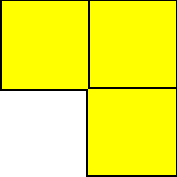
\includegraphics{induction-09-yellowtromino} \qquad \qquad 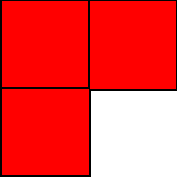
\includegraphics{induction-10-redtromino}
% \end{center}
\vspace{-2pt}
		
	\begin{itemize}
	 	\item Place a single tromino (yellow in the picture) so that one of its squares lies in each remaining quadrant. What's left of each quadrant is a $2^1\times 2^1$ grid with one missing square: again tilable.
	\end{itemize}
	
	This scratch work is really an argument $P(1)\Longrightarrow P(2)$! It remains only to formalize this intuition into a general proof. We proceed by induction on $n$.
	\begin{description}
		\item[\normalfont\emph{Base case} ($n=1$):] If a single square is removed from a $2\times 2$ grid, the three remaining squares form single L-shaped tromino.
		\item[\normalfont\emph{Induction step}:] Fix $n\in\N$ and assume that after removing \emph{any} square from any $2^n\times 2^n$ grid, the remainder is tilable. Now take any $2^{n+1}\times 2^{n+1}$ grid and remove a square.
	\begin{itemize}
	  \item By the induction hypothesis, the $2^n\times 2^n$ quadrant with the removed square is tilable.
	  \item Place a single tromino in the center so that one of its squares lies in each remaining quadrant. What's left of each quadrant is a $2^n\times 2^n$ grid with one missing square: again tilable by the induction hypothesis.
	\end{itemize}  
	\end{description}
	By induction, we conclude that every $2^n\times 2^n$ grid is tilable by trominos after any square is removed.
\end{example}


\goodbreak

\begin{exercises}{}{}
	A reading quiz and several questions with linked video solutions can be found \href{http://www.math.uci.edu/~ndonalds/math13/selftest/5-1-induction.html}{online}.

	\begin{enumerate}
	  \item Suppose you can move one disk on the Tower of Hanoi per second.
	  \begin{enumerate}
	    \item One of the oldest versions of the problem has monks transferring a tower of 64 disks. Roughly how many years would this take?
	    \item In a realistic human lifetime, how large a tower could be moved?
	  \end{enumerate}
	  
	  
	  \item Imagine you cut a large large piece of paper in half and stack the two pieces on top of each other. You then repeat the process, cutting all sheets in half and making a single taller stack.
		\begin{center}
			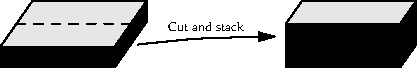
\includegraphics{induction-02-paper}
		\end{center}
		If a single sheet of paper has thickness $0.1$\,mm, how many times would you have to repeat the cut-and-stack process until the stack of paper reached to the sun? ($\approx 150$ million kilometers). \emph{Prove} that you are correct.
	  
	
	  \item A room contains $n$ people. Everybody wants to shake everyone else's hand (but not their own).
	  \begin{enumerate}
	    \item Suppose $n$ people require $h_n$ handshakes. If person $n+1$ enters the room, how many \emph{additional} handshakes are required? Obtain a recurrence relation for $h_{n+1}$ in terms of $h_n$.
	    \item Hypothesize a general formula for $h_n$, and prove it by induction.
	  \end{enumerate}
	  
	%   \item Skippy the Kangaroo is playing jump rope, but he tires as the day goes on. The heights $h_n$ (inches) of successive jumps are related by the recurrence 
	%   \[h_{n+1}=\frac 8{9} h_n+1.\]
	%   \begin{enumerate}
	%   	\item Suppose that Skippy's initial jump has height $h_1=100\,$in. Show that Skippy fails to jump above 10in for the first time on the 40th jump.
	%   	\item Find the \emph{total} height jumped by Skippy in the first $n$ jumps.
	%   \end{enumerate}
	%   \emph{You may find it useful to define $H_n=h_n-9$ and think about the recurrence for $H_n$. Now guess and prove a general formula for $H_n$. Finally, remind yourself about geometric series.})
	  
	  
	  \item\begin{enumerate}
	    \item In Example \ref*{ex:ind2}.\ref{ex:ind22}, what is the proposition $P(n+1)$?
	    \item In the induction step of Example \ref*{ex:ind2}.\ref{ex:ind22}, explain why it would be incorrect to write
	    \begin{align*}
				P(n+1)-P(n)&=(n+1)\bigl[(n+2)(2n+3)-n(2n+1)\bigr]\\
				&=(n+1)(2n^2+7n+6-2n^2-n)\\
				&=6(n+1)^2
			\end{align*}
			\item Extend the Example by proving, by induction, that $\sum\limits_{k=1}^nk^2=\frac 16n(n+1)(2n+1)$.
	  \end{enumerate}
  
  
	  \item Prove by induction that for each natural number $n$, we have $\smash{\sum\limits_{k=0}^n2^k=2^{n+1}-1}$.
		
		
		\item Consider the statement: If $n$ is a natural number, then $\smash{\sum\limits_{k=1}^nk^3=\frac 14n^2(n+1)^2}$
		\begin{enumerate}
		  \item What, explicitly, is $\smash{\sum\limits_{k=1}^4k^3}$?
		  \item What would be meant by the expression $\smash{\sum\limits_{k=1}^nn^3}$, and why is it different to $\smash{\sum\limits_{k=1}^nk^3}$?
		  \item Proof the statement by induction.
	  \end{enumerate}
	
	
  	\item\begin{enumerate}
    	\item Prove by induction that $\forall n\in\N$ we have $3\mid(2^n+2^{n+1})$.
    	\item Give a direct proof that $3\mid(2^n+2^{n+1})$ for all integers $n\ge 1$.
  	\end{enumerate}

  
		\item Prove \emph{by induction} that for every $n\in\N$ we have $n\equiv 5$ or $n\equiv 6$ or $n\equiv 7\spmod 3$.
	
		\item Prove by induction that, for all $n\in\N$,
		\[
			1\cdot 2+2\cdot 3+3\cdot 4+\cdots +n(n+1) =\frac 13n(n+1)(n+2)
		\]

		\item\begin{enumerate}
		  \item Show, by induction, that for all $n\in\N$, the number 4 divides the integer $11^n-7^n$.
			\item More generally, prove by induction that $(a-b)\mid (a^n-b^n)$ for any $a,b,n\in\N$.
		\end{enumerate}
	
	
 		%\item Prove by induction that for all $k \in \N$, we have $8^k-1$ divisible is a multiple of $7$. 
	
	
		\item\begin{enumerate}
		  \item Find a formula for the sum of the first $n$ odd natural numbers. Prove your assertion.
		 	\item Use Theorem \ref{thm:ind1} to give an alternative direct proof of your formula.
		\end{enumerate} 
  

		\item Find the error in the following ``proof'' of the statement, ``All cats have the same color fur.''
		\begin{proof}
	    Let $P(n)$ be the proposition, ``Any set of $n$ cats have the same color fur.'' We prove by induction on $n$. 
	    \begin{description}\itemsep0pt
	    	\item[\normalfont\emph{Base case} ($n=1$):] Any cat has the same color fur as itself.
	    	\item[\normalfont\emph{Induction step}:] Fix $n\in\N$ and assume $P(n)$. Take any set $S= \{C_1,C_2,\ldots,C_{n+1}\}$ of $n+1$ cats. The set $S\setminus\{C_1\}$ has $n$ cats; by the induction hypothesis all have the same color fur. Again by the induction hypothesis, all cats in $S\setminus\{C_2\}$ have the same color fur. Combining these observations, we see that all cats in $S$ have the same color fur. Since $S$ was arbitrary, we see that $P(n+1)$ holds.
	    \end{description}
	    By induction, $P(n)$ is true for all $n\in\N$, which establishes the claim.
		\end{proof}

		\item Use induction, the product rule, and the fact that $\diff xx=1$ to prove the power law from calculus:
		\[
	    \forall n\in\N,\ \diff x x^n =nx^{n-1}
		\]


		\item A (real) \emph{polynomial} of degree $n$ is a function $p(x)=a_nx^n+a_{n-1}x^{n-1}+ \cdots +a_1x+a_0$, whose \emph{coefficients} $a_k$ are real numbers and where $a_n\neq 0$.
		\begin{enumerate}
    	\item Prove: for all $n\in\N$,
    	\[
        \diff[{}^n]{x^n} e^{x^2} = p_n(x) e^{x^2}
    	\]
    	where $p_n(x)$ is some polynomial of degree $n$.

			\item (Hard)\lstsp Let $p(x)$ be a polynomial of degree $n\ge 1$. Show $p$ has at most $n$ roots.\par
			(\emph{Hint: induct on the degree $n$})
		\end{enumerate}


		\item Consider the following scratch work. Determine what result is being proved, then convert the scratch work into a formal proof of that result.
	  \begin{align*}
	    (1+x)^{n+1}&=(1+x)^n(1+x)\ge (1+nx)(1+x)\\
	    &=1+x+nx+nx^2=1+(n+1)x+nx^2\\
	    &\ge 1+(n+1)x
	  \end{align*}

	\end{enumerate}

\end{exercises}

\clearpage



\subsection{Well-ordering and the Principle of Mathematical Induction}\label{sec:wellorder}


In this section we think more carefully about the logic behind induction, by tying it to a fundamental property of the natural numbers.

\begin{defn}{}{wellorder}
	A non-empty set of real numbers $A$ is \emph{well-ordered} if every non-empty subset of $A$ contains a minimum element.
\end{defn}

To test if a set $A$ is well-ordered, we need to check \emph{all} of its non-empty subsets. The definition could be written as equivalently as follows, where in the second line we expand what is meant by a \emph{minimum}:
\begin{itemize}
  \item $\forall B\subseteq A$ such that $B\neq\emptyset$, $\min B$ exists.
  \item $\forall B\subseteq A$, $B\neq\emptyset\implies \exists b\in B$ such that $\forall x\in B$, $b\le x$.
\end{itemize}
To show that $A$ is \emph{not} well-ordered, we need only exhibit a non-empty subset $B$ with \emph{no minimum.}

\begin{examples}{}{}
	\exstart $A=\{4,-7,\pi,19,\ln 2\}$ is a well-ordered set. There are 31(!) non-empty subsets of $A$, each of which has a minimum element.\vspace{-5pt}
	\begin{enumerate}\setcounter{enumi}{1}
	  \item[] Can you justify this fact \emph{without} listing the subsets? It might be easier to think about why any \emph{finite} set $A=\{a_1,\ldots,a_n\}\subseteq\R$ is well-ordered\ldots 
	  
	  \item The interval $A=[3,10)$ is not well-ordered. Indeed $B=(3,4)$ is a non-empty subset which has no minimum element. While you should believe this, let's prove it anyway!\par
	  We need to prove that $\forall b\in B, \exists x\in B$ with $x>b$. Given any $b\in(3,4)$, observe that $x:=\frac{b+3}2$ satisfies
	  \[
	  	3<x<b<4 \quad\text{from which}\quad x\in B\text{ and }x<b
	  \]
	  You could also argue by contradiction (if $b\in B$ is $\min B$, then\ldots).
	  
	  \item The integers $\Z$ are not well-ordered. For instance, $\Z$ is a non-empty subset of itself and there is no minimum integer.
	\end{enumerate}
\end{examples}

You might suspect (wrongly!) that every well-ordered set is finite. That the natural numbers form a well-ordered \emph{infinite} set is, for us, an axiom:
\footnote{There are many ways to define the natural numbers. Typically well-ordering is either an axiom (essentially part of the definition) or a theorem. Compare with Exercise \ref{exs:peano} for an alternative approach.} a foundational claim that forms part of our basic conception of the natural numbers.

\begin{axiom}{Well-ordering Principle}{}
	$\N$ is well-ordered.
\end{axiom}


Also known as the \emph{least natural number principle}, the well-ordering principle is used repeatedly in mathematics. In fact we've already done so in this text! Consider the set of positive remainders generated by the Euclidean algorithm (Theorem \ref{thm:euclidalg}) applied to $a>b\in\N$:
\[
	\{\ldots,r_2,r_1,b,a\}\subseteq\N
\]
Well-ordering guarantees that this set has a minimal element $r_t$ (which turns out to be $\gcd(a,b)$); this is essentially the argument for Exercise \ref*{sec:gcd}.\ref{exs:euclidalgproof}(a).

\goodbreak  

%  When written in roster notation in increasing order, any set that `looks like' $\N$, is also well-ordered. For example
% \[
% 	A=\left\{0,\frac 12,\frac 23,\frac 34,\frac 45,\ldots\right\}=\left\{\frac n{n+1}:n\in\N\right\}
% \]
Armed with this axiom, we can justify the method of proof by induction. 

\begin{thm}{Principle of Mathematical Induction}{ind}
	For each $n\in\N$, let $P(n)$ be a proposition. Additionally make the two standard assumptions for induction:
	\begin{quote}
		\emph{Base case}:\lstsp $P(1)$ is true\par
		\emph{Induction step}:\lstsp $\forall n\in\N,\ P(n)\Longrightarrow P(n+1)$
	\end{quote}
	Then $P(n)$ is true for all $n\in\N$.
\end{thm}

Before attempting a proof, consider how the theorem could be written as a pure implication:
\[
	\textcolor{blue}{P(1)\wedge\bigl(\forall n\in\N,P(n)\Longrightarrow P(n+1)\bigr)}\Longrightarrow \textcolor{Green}{\bigl(\forall n\in\N, P(n)\bigr)}
\]
This helps us select a proof strategy: a direct approach seems hard since the \textcolor{Green}{conclusion} is universal; a contrapositive approach requires an ugly negation of the \textcolor{blue}{hypothesis}; a proof by contradiction seems most sensible since negation of the \textcolor{Green}{conclusion} is straightforward.

\begin{proof}
	We argue by contradiction. Assume the base case, the induction step, and that $\exists n\in\N$ for which $P(n)$ is \emph{false.} The set of natural numbers
	\[
		S:=\bigr\{k\in\N:P(k)\text{ is false}\bigr\}
	\]
	is non-empty (since $n\in S$). Well-ordering guarantees that $s:=\min S$ exists. Observe:
	\begin{itemize}\itemsep0pt\parskip2pt
	  \item $s\in S\Longrightarrow$ \textcolor{red}{$P(s)$ is \emph{false}}.
	  \item The \emph{base case} tells us that $s\neq 1$, whence $s-1\in\N$.
	  \item $s-1<\min S\implies P(s-1)$ is \emph{true.}
	  \item The \emph{induction step} ($P(s-1)\Longrightarrow P(s)$) tells us that \textcolor{red}{$P(s)$ is \emph{true}}.
	\end{itemize}
	\textcolor{red}{Contradiction}: $P(s)$ cannot be both true and false!
\end{proof}


Now we have the proof, it is straightforward to extend the principle of induction. For any integer $m$ (positive, negative or zero), the set
\[
	\Z_{\ge m}=\{n\in\Z:n\ge m\}=\{m,m+1,m+2,m+3,\ldots\}
\]
is also well-ordered. By changing the base case to $P(m)$ and replacing $\N$ with $\Z_{\ge m}$, we immediately obtain the proof of a more general principle of induction.

\begin{cor}{Induction with base case $m$}{}
	Fix an integer $m$. For each integer $n\ge m$, let $P(n)$ be a proposition. Suppose:
	\begin{quote}
		\emph{Base case}:\lstsp $P(m)$ is true\par
		\emph{Induction step}:\lstsp $\forall n\in\Z_{\ge m},\ P(n)\Longrightarrow P(n+1)$
	\end{quote}
	Then $P(n)$ is true for all $n\in\Z_{\ge m}$.
\end{cor}

The intuitive concept is exactly as before, just with a different base case!
\[
	P(m)\implies P(m+1)\implies P(m+2)\implies P(m+3)\implies\cdots
\]
\goodbreak

% As long as you explicitly prove the first claim in the sequence, and you show the induction step, then all the propositions are true.\par



\begin{examples}{}{}
	\exstart For all integers $n\ge 2$, we have\footnotemark
	\[
		\sum\limits_{k=2}^n\frac 1{k(k-1)} =1-\frac 1n\tag{$\ast$}
	\]	
	\begin{enumerate}\setcounter{enumi}{1}
		\item[]\begin{description}
			\item[\normalfont\emph{Base case} ($n=2$):] When $n=2$, ($\ast$) reads $\smash{\sum\limits_{i=2}^2}\frac 1{i(i-1)}=\frac 12=1-\frac 12$.
			\item[\normalfont\emph{Induction step}:] Assume that ($\ast$) is true for some fixed $n\ge 2$. Then
			\begin{align*}
				\sum_{i=2}^{n+1}\frac 1{k(k-1)} &=\sum_{i=2}^{n}\frac 1{k(k-1)}+\frac 1{(n+1)n} =1-\frac 1n+\frac 1{n(n+1)}\tag{induction hypothesis}\\
				&=1-\frac{(n+1)-1}{n(n+1)} =1-\frac 1{n+1}
			\end{align*}
			which is exactly ($\ast$) when $n$ is replaced by $n+1$.
		\end{description}
		By induction ($\ast$) holds for all integers $n\ge 2$.
	
	  \item For all integers $n\ge 4$, we claim that $3^n>n^3$.\par
	  We really need a different base case: when $n=3$, the claim $3^3>3^3$ is false! As is often the case, it helps to do some scratch work first. The \textcolor{blue}{induction hypothesis} allows us to see that 
	  \[
	  	3^{n+1}=3\cdot \textcolor{blue}{3^n} >3 \textcolor{blue}{n^3}
	  \] 
	  The proof of the induction step therefore hinges on being able to show that $3n^2\ge (n+1)^3$. There are many ways to convince yourself of this: for instance
	  \[
	  	3n^3\ge(n+1)^3\iff 3\ge\left(\frac{n+1}n\right)^3 =\left(1+\frac 1n\right)^3 \tag{$\dag$}
	  \]
	  The right side \emph{decreases} as $n$ increases; since $n\ge 4$, the right side is at most $\left(\frac 54\right)^3=\frac{125}{64}<2$, whence ($\ast$) holds for all $n\ge 4$.\smallbreak
	  
	  We now prove the original claim by induction.	  
	  \begin{description}
	  	\item[\normalfont\emph{Base case} ($n=4$):] Observe that $3^4=81>64=4^3$.
	  	\item[\normalfont\emph{Induction step}:] Fix $n\in\Z_{\ge 4}$ and suppose that $3^n>n^3$. By ($\dag$), we see that
			\[
				3^{n+1}=3\cdot 3^n>3n^3\ge (n+1)^3
			\]
	  \end{description}
	  By induction, we conclude that $3^n>n^3$ whenever $n\in\Z_{\ge 4}$.
	\end{enumerate}
\end{examples}


\footnotetext{You might have encountered this example as a \emph{telescoping series} in calculus:
\[
	\sum\limits_{k=2}^n\frac 1{k(k-1)}=\frac 1{2\cdot 1}+\frac 1{3\cdot 2}+\cdots +\frac 1{n(n-1)} =\left(1-\frac 12\right) +\left(\frac 12-\frac 13\right) +\cdots +\left(\frac 1{n-1}-\frac 1n\right) =1-\frac 1n
\]
In calculus, you'd take the limit as $n\to\infty$ to obtain the infinite series $\sum\limits_{k=2}^\infty\frac 1{k(k-1)}=1$}


As a final example, we prove an extended version of de Morgan's law for sets (Theorem \ref{thm:setcomp}(a)).

\begin{example}{}{}
	For any collection of sets $A_1,\ldots,A_n$ where $n\ge 2$, we have
	\[
	 	\comp{(A_1\cap \cdots\cap A_n)}=\comp{A_1}\cup\cdots\cup\comp{A_n} \tag{$\ddag$}
	\]
	\begin{description}
		\item[\normalfont\emph{Base case} ($n=2$):] $\comp{A_1\cap A_2}=\comp{A_1}\cup\comp{A_2}$ is precisely the standard de Morgan identity.
		\item[\normalfont\emph{Induction step}:] Fix $n\in\N_{\ge 2}$ and suppose ($\ddag$) holds for \emph{all} collections of $n$ sets. Given a collection of $n+1$ sets, we see that
		\begin{align*}
			\comp{(A_1\cap \cdots\cap A_n\cap A_{n+1})} &=\comp{\bigl((A_1\cap \cdots\cap A_n)\cap A_{n+1}\bigr)}\\
			&=\comp{(A_1\cap \cdots\cap A_n)}\cup \comp{A_{n+1}} \tag{de Morgan again!}\\
			&=\comp{A_1}\cup\cdots\cup\comp{A_n}\cup\comp{A_{n+1}} \tag{induction hypothesis}
		\end{align*}
	\end{description}
	By induction the claim ($\ddag$) holds for any collection of $n$ sets.
\end{example}

We could have approached the argument as a standard induction with base case $n=1$. Instead we deliberately chose the base case $n=2$, both to avoid confusion (the trivial $\comp{A_1}=\comp{A_1}$ isn't helpful or interesting) and to highlight the importance of de Morgan's law for two sets to the entire argument.

\boldsubsubsection{Proof by Minimal Counter-example}

Sometimes authors present induction arguments as contradiction proofs in line with Theorem \ref{thm:ind}: the element $s=\min S$ is known as the \emph{minimal counter-example.} Here are two variations on this idea; the first is a straight translation of an induction where the base case and induction step are clear.

\begin{examples}{}{}
	\exstart We prove: for all $n\in\N_0$, $\sum\limits_{k=0}^n 2^k=2^{n+1}-1$.\vspace{-10pt}
	
	\begin{enumerate}\setcounter{enumi}{1}
	  \item[]Suppose to the contrary and let $s\ge 0$ be the minimal counter-example.
	  \begin{itemize}
	    \item Since $\smash{\sum\limits_{k=0}^0} 2^k=2^0=1=2^{0+1}-1$, we see that $s\neq 0$.\hfill (\emph{base case})
	    \item But then
	    \[
	    	\sum\limits_{k=0}^s2^k=2^s+\sum\limits_{k=0}^{s-1} 2^k =2^s+2^s-1=2^{s+1}-1 \tag{\emph{induction step}}
	    \]
	    contradicts the fact that $s$ is a counter-example!
	  \end{itemize} 
	  
	  
	  \item We re-prove Theorem \ref{thm:sqrt2}: $\sqrt 2\notin\Q$. Suppose $\sqrt 2$ is rational and consider the set
	  \[
	  	S=\bigl\{x\in\N:\exists y\in \N\text{ with }x^2=2y^2\bigr\}
	  \]
	  Let $s=\min S$ and $t\in\N$ be such that $s^2=2t^2$: plainly $\textcolor{red}{t<s}$. Since $s^2$ even $\Longrightarrow s$ even, we can write $s=2k$, from which
	  \[
	  	4k^2=2t^2\implies n^2=2k^2\implies \textcolor{red}{t\in S}
	  \]
	  This contradicts the minimality of $m$.\par
	  This approach is often used in number theory in the guise of Fermat's \emph{method of infinite descent.}
	\end{enumerate}
\end{examples}

\iffalse

Our final example involves a little abstraction.

\begin{thm}{}{polygon}
	The interior angles of an $n$-gon ($n$-sided polygon) sum to $180(n-2)$ degrees.
\end{thm}

We will take the initial case ($n=3$) that the angles of a triangle sum to \ang{180} as given (can you prove it?) and merely prove the induction step. The main logical difficulty is that we must consider \emph{all} $n$-gons simultaneously. If we were to write the induction step in the form
\[
	\forall n\in\Z_{\ge 3},\ P(n)\implies P(n+1)
\]
then the proposition $P(n)$ would be
\[
	P(n):\quad \forall n\text{-gons }\cP_n,\text{ the sum of the interior angles of $\cP_n$ is $180(n-2)$\textdegree}
\]
To prove our induction step for a \emph{fixed} integer $n$, we must show that \emph{all} $(n+1)$-gons have the correct sum of interior angles. We therefore assume that we are given some $(n+1)$-gon $\cP_{n+1}$ and proceed to compute its interior angles in terms of a related $n$-gon.

\begin{proof}
	Fix an integer $n\ge 3$, and suppose that \emph{all} $n$-gons have interior angles summing to $180(n-2)$\textdegree. Suppose we are given an $(n+1)$-gon $\cP_{n+1}$. Select any vertex $A$ and label the adjacent vertices $B$ and $C$. Delete $A$, and join $B$ and $C$ with a straight edge. The result is an $n$-gon $\cP_n$. There are two cases to consider.\footnotemark{}\par

	\begin{minipage}[t]{0.64\linewidth}\vspace{0pt}
		Case 1: The deleted point $A$ is \emph{outside} $\mathcal{P}_n$. The sum of the interior angles of $\mathcal{P}_{n+1}$ exceeds those of $P_n$ by $\alpha+\beta+\gamma=180$\textdegree. Therefore $\mathcal{P}_{n+1}$ has interior angles summing to $180(n-2)\text{\textdegree}+180\text{\textdegree}=180[(n+1)-2]$\textdegree.\par
	
		Case 2: The deleted point $A$ is \emph{inside} $\mathcal{P}_n$. To obtain the sum of the interior angles of $\mathcal{P}_{n+1}$, we take the sum of the interior angles of $\mathcal{P}_n$ and do three things:
		\begin{itemize}\setlength{\itemsep}{0pt}
	  	\item \emph{Subtract} $\beta$
	  	\item \emph{Subtract} $\gamma$
	  	\item \emph{Add the reflex angle $360$\textdegree$-\alpha$ at $A$}
		\end{itemize}
		We are therefore adding an additional
		\[
			-\beta-\gamma+(360\text{\textdegree}-\alpha)=360\text{\textdegree}-(\alpha+\beta+\gamma)=180\text{\textdegree}
		\]
	\end{minipage}
	\hfill
	\begin{minipage}[t]{0.35\linewidth}\vspace{0pt}
		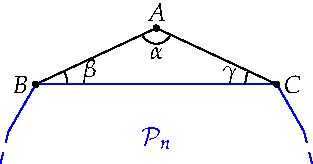
\includegraphics[width=\textwidth]{induction-05-polygon}\\
		Case 1: $A$ outside $\mathcal{P}_n$\\[25pt]
		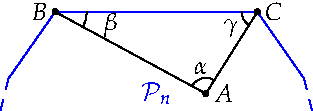
\includegraphics[width=\textwidth]{induction-06-polygon}\\
		Case 2: $A$ inside $\mathcal{P}_n$
	\end{minipage}\\[8pt]
	$\mathcal{P}_{n+1}$ again has interior angles summing to $180[(n+1)-2]$\textdegree.
\end{proof}

\footnotetext{We are obscuring two subtleties here. It is a fact, though not an obvious one, that it is always possible to choose a vertex $A$ so that the new polygon $\cP_n$ doesn't cross itself. Read about `ears' and `mouths' of polygons and triangulation if you're interested. There are also two other, less likely, cases which we didn't consider: when deleting a point from an ($n+1$)-gon it is possible to obtain  an $(n-1)$-gon, or even an $(n-2)$-gon. To think it out, try drawing a 12-gon in the shape of a Star of David. Deleting one of the outer corners creates a 9-gon! Dealing with these cases strictly requires strong induction, so we return to them later.}

\fi

%Wellorder stuff!
%     \item Prove: $n! \le \left(\frac{n + 1}{2}\right)^n$.\par
%      (\emph{Hint: find a formula for the sum of the first $n$ positive integers})
%   


% \subsubsection*{Optional: Density of the Rationals}
% 
% In our last example, we offer a more direct application of $\N$ being well-ordered. One of the  key properties of the rational numbers $\Q$ is their density in the real line. Intuitively, the idea is that no matter how close you "zoom in" on the real line, you can always locate a rational number. We formalize this with the following definition.
% 
% \begin{defn}
% We say a set $A \subseteq \R$ is \textbf{dense} (in $\R$) if for any real numbers $x$ and $y$ such that $x < y$, there is  $a \in A$ such that $x < a < y$.
% \end{defn}
% 
% So if you take two real numbers, you can always find an element from $A$ in between them, no matter how close the two real numbers are from each other. Our goal will be to prove that the rational numbers $\Q$ are dense in $\R$. For this, we will use the well-orderedness of $\N$ along with the following:
% 
% \begin{axiom}
% The real numbers $\R$ have the \textbf{Archimedean property}, that is, for any real numbers $x,y > 0$, there is $n \in \N$ such that $nx > y$.
% \end{axiom}
% 
% It is not really necessary to take this as an axiom as the Archimedean property of $\R$ can be proved from more basic principles. However, this requires some knowledge about how to construct the real numbers which lies beyond the scope of this course. Back to our goal, we need the following lemma which states that if two real numbers differ by more than $1$, then there must be an integer between them.
% 
% \begin{lemm}\label{lemm:rationaldensityprep}
% Suppose we have $x,y \in \R$ with $y - x > 1$. Then there exists $k \in \Z$ such that $x < k < y$.
% \end{lemm}
% 
% \begin{proof}
% The idea is to take $k$ to be the least integer greater than $x$. We will show such an integer exists using the fact that $\N$ is well-ordered. Let $A = \{n \in \Z : n > x\}$. Then $A \neq \emptyset$ by the Archimedean property (why?). Let $m \in \Z$ be a number such that $m < x$ (this is another application of the Archimedean property), and thus $m < n$ for all $n \in A$, by definition of $A$. Let 
% \[
% S = \{n - m + 1 : n \in A\}.
% \]
% So $S \subseteq \N$ and since $A \neq \emptyset$, we have $S \neq \emptyset$. Since $\N$ is well-ordered, $S$ has  a minimum element $s$. Then $k = s + m - 1$ is the minimum element of $A$ (why?).
% 
% By definition $x < k$. But by minimality of $k$, $k - 1 \notin A$, i.e., $x \geq k - 1$. Thus $x < k \leq x + 1$. Finally, since $y - x > 1$, we have $x + 1 < y$. All together, $x < k \leq x + 1 < y$. So $k$ is as required.
% \end{proof}
% 
% Now we can prove our main result.
% 
% \begin{thm}
% The rational numbers $\Q$ are dense in $\R$.
% \end{thm}
% 
% \begin{proof}
% Let $x,y \in \R$ with $x < y$ be arbitrary. We need to find $r \in \Q$ with $x < r < y$. Then $y - x > 0$. By the Archimedean property, there is $n \in \N$ such that $n(y - x) > 1$. Since $ny - nx > 1$, we can apply Lemma \ref{lemm:rationaldensityprep} to get $k \in \Z$ such that $nx < k < ny$. As $n \geq 1 > 0$, dividing yields $x < \frac{k}{n} < y$. Take $r = \frac{k}{n} \in \Q$.
% \end{proof}

% \begin{aside}{}{}
% 	{\bf Well-ordering more generally}
% 	
% 	Well-ordering is a fundamental concept whose implications are far beyond what we're discussing here. Informally speaking, \emph{well-ordering} a set $A$ involves listing the elements of $A$ in some order so that every non-empty subset of $A$ has a first element \emph{with respect to that order.}\\
% 	Consider, for example, the set of negative integers $\Z^-$. For the purposes of these notes we will always consider the standard ordering:
% 	\[
% 		\cdots<-4<-3<-2<-1
% 	\]
% 	Written in the standard order, $\Z^-=\{\ldots,-4,-3,-2,-1\}$ is \emph{not} a well-ordered set. In a more advanced discussion, one could consider alternative orderings, and the definition of well-ordered would change accordingly. If we choose the ordering
% 	\[
% 		\Z^-=\{-1,-2,-3,-4,\cdots\},\tag{$\ast$}
% 	\]
% 	then $\Z^-$ would be well-ordered: if $B\subseteq\Z^-$ is non-empty and has its elements listed in the same order as $(\ast)$, then $B$ has a first element. With a little thinking, we could modify the proof of the principle of mathematical induction to allow us to prove theorems of the form $\forall n\in\Z^-,\ P(n),$ by induction. The base case is $n=-1$ and the induction step justifies the chain
% 	\[
% 		P(-1)\implies P(-2)\implies P(-3)\implies\cdots
% 	\]
% 	An extremely important theorem in advanced set theory states that it is possible to well-order \emph{every} set. With a slight modification of the process, this massively increases the applicability of induction. In these notes we keep things simple: well-ordering is always in the sense of Definition \ref{defn:wellorder}, where we list the elements of a set in the usual increasing order. For a more esoteric example of a well-ordered set, see the final Exercise below.
% \end{aside}


\begin{exercises}
	A reading quiz and several questions with linked video solutions can be found \href{http://www.math.uci.edu/~ndonalds/math13/selftest/5-2-wellorder.html}{online}.

	\begin{enumerate}
  	\item Prove that the interval $(-2,5]$ has no minimum element.
  
  	\item\begin{enumerate}
    	\item Suppose that $n\ge 3$. Prove that $\left(\frac{n+1}n\right)^2<2$.
    	\item Hence or otherwise, prove that $n^2<2^n$ for all natural numbers $n\ge 5$.
  	\end{enumerate}
  	
  	
%   	\item Prove the second extended de Morgan result: for any sets $A_1,\ldots,A_n$,
%   	\[
%   		\comp{(A_1\cup\cdots \cup A_n)} =\comp{A_1}\cap\cdots\cap\comp{A_n}
%   	\]


	  \item Consider the following result. For every natural number $n\ge 2$,
		\[
			\left(1-\frac{1}{4}\right) \left(1-\frac{1}{9}\right) \left(1-\frac{1}{16}\right) \cdots \left(1-\frac{1}{n^2}\right) = \frac{n+1}{2n}
		\]
	  \begin{enumerate}
	    \item If the statement is written in the form $\forall n\in\N_{\ge 2},\ P(n)$, what is the proposition $P(n)$?
% 	    \item $\Pi$-notation is used for products in the same way as $\Sigma$-notation for sums: for example
% 	    \[\prod_{k=1}^5(k+1)^k=2^1\cdot 3^2\cdot 4^3\cdot 5^4\cdot 6^5\]
% 	    Rewrite the statement using $\Pi$-notation.
	    \item Prove the result by induction.
	  \end{enumerate}
	  
	  
	
		\item Prove the geometric series formula: if $r\neq 1$ and $n\in\N_0$, then
			$\sum\limits_{k=0}^nr^k=\frac{1-r^{n+1}}{1-r}$
			
		
		\item For all integers $n\ge 3$, prove that $\sum\limits_{k=3}^n\frac 1{k(k-2)} =\frac 34-\frac{2n-1}{2n(n-1)}$	
	
	
  	\item The set $A_3=\{1,2,3\}$ satisfies the property that the sum of its elements (6) is divisible by every element.
  	\begin{enumerate}
  	  \item Use induction to prove that for any $n\ge 3$, there is a set $A_n$ consisting of $n$ natural numbers such that the sum of the numbers in $A_n$ is divisible by every element of $A_n$.
  	  \item Prove that no set of \emph{two} natural numbers satisfies the property.
  	\end{enumerate}
 
	
		\item For each $n\in\N$, let $P(n)$ and $Q(n)$ be propositions.
		\begin{enumerate}
			\item Let $s$ be the smallest natural number such that $P(s)$ is false. What can you say about the elements of the set $A=\{n\in\N:n<s\}$ with respect to the property $P$?
			\item Let $a$ be minimal such that $P(a)\vee Q(a)$ is false. What can you say about the elements of the set $B=\{n\in\N:n<a\}$ with respect to the properties $P$ and $Q$?
			\item Let $u$ be minimal such that $P(u)\wedge Q(u)$ is false. What can you say about the elements of the set $C=\{n\in\N:n<u\}$ with respect to the properties $P$ and $Q$?
			\item Assume that $P(1)$ is true, but that ``$\forall n\in\N,\ P(n)$'' is false. Show that there exists a natural number $k$ such that the implication $P(k)\Longrightarrow P(k+1)$ is false.
		\end{enumerate}
	
		
	
		\item Prove that if $A\subseteq\R$ is a \emph{finite} set, then $A$ is well-ordered.
	
	
		\item Prove that $\Q$ is not well-ordered.
  
	
		\item We use the fact that $\N_0$ is well-ordered to prove the division algorithm (Theorem \ref{thm:div}).
		\begin{quote}
			\emph{If $m\in\Z$ and $n\in\N$, then $\exists$ unique $q,r\in\Z$ such that $m=qn+r$ and $0\le r<n$.}
		\end{quote}
	
		Given $m,n$, define $S=\bigl\{k\in\N_0:k=m-qn\text{ for some }q\in\Z\bigr\}$.	
		\begin{enumerate}
			\item (Existence)\lstsp Show that $S$ is a \emph{non-empty} subset of $\N_0$. By well-ordering, \emph{define} $r:=\min S$. Prove that $0\le r<n$.
			\item (Uniqueness)\lstsp Suppose two pairs of integers $(q_1,r_1)$ and $(q_2,r_2)$ satisfy $m=q_in+r_i$ and $0\le r_1,r_2<n$. Prove that $r_1=r_2$.
		\end{enumerate}
		
		
		



	
	\item Prove: for any $n\in\N$, $\sum\limits_{i=1}^n\frac{1}{i^2}<2$\par
	(\emph{Hint: prove the stronger fact that $\smash{\sum\limits_{i=1}^n} \frac{1}{i^2} < 2 - \frac{1}{n}$ for all $n \ge 2$})
		
	
  \item\label{exs:peano} (Hard)\lstsp We consider a slimmed-down version of Peano's axioms for the natural numbers.
	\begin{itemize}
		%\item[i.] (\emph{Initial element})\lstsp $1\in\N$
		\item[i.] (\emph{Successor/unique predecessor})\lstsp $\exists f:\N\to\N$ injective. We write this as $f(n)=n+1$, so
		\[
			n\in\N\Longrightarrow n+1\in\N\quad\text{and}\quad m+1=n+1\implies m=n
		\]
		\item[ii.] (\emph{Initial element})\lstsp $1\in\N$ and $1\notin\range(f)$: there is no $x\in\N$ for which $x+1=1$.
		%\item[ii.] (\emph{No predecessor of the initial element})\lstsp $1\not\in\range(f)$
		%\item[iv.] (\emph{Unique predecessor/order})\lstsp $f$ is injective: $m+1=n+1\implies m=n$
		\item[iii.] (\emph{Induction})\lstsp Any subset $A\subseteq\N$ with the following properties \emph{equals} $\N$:\footnotemark
		\[
			1\in A\quad\text{and}\quad \forall a\in A,\ a+1\in A
		\]
	\end{itemize}
	\begin{enumerate}
		\item Replace $\N$ with $\Z$ in each axiom. Which are true and which false?
		\item Let $T=\bigl\{(m,n):m,n\in\N\bigr\}$ be the set of all ordered pairs of natural numbers.
		\begin{enumerate}
		  \item Let $f:T\to T$ be the function $f(m,n)=(m+1,n)$. Letting the pair $(1,1)$ play the role of 1, and $f$ the successor function, decide which of Peano's axioms are satisfied by $T$.
			\item Repeat the question for the same initial element and 
			\[
				f:T\to T:(m,n)\mapsto
				\begin{cases}
					(m-1,n+1)&\text{if }m\ge 2\\
					(m+n,1)&\text{if }m=1
				\end{cases}
			\]
		\end{enumerate}
		
		\item Prove that $\range(f)=\N\setminus\{1\}$: every element except 1 is the successor of something.\par
		(\emph{Hint: let $A=\{1\}\cup\range(f)$ in the induction axiom)}
		
		
		\item For $x,a\in\N$ we say that $x<a$ if $a=f(f(\cdots f(f(x))\cdots)) =(\cdots((x+1)+1)\cdots)+1$.
		\begin{enumerate}
		  \item Prove that $a<a$ is a contradiction.
		  \item Prove that $\N$, as defined by Peano, is well-ordered.\par
			(\emph{Hint: if $B\subseteq\N$ is non-empty, consider $A:=\{x\in\N:\forall b\in B, x<b\}$})
		\end{enumerate}

	\end{enumerate}
	
% 	\item (\emph{Ignore this question if you haven't studied matrices}) Suppose that $A=\begin{smatrix}7&12\\-2&-3\end{smatrix}$. We prove that
% 	\[\forall n\in\Z,\quad A^n=\begin{pmatrix}-2&-6\\1&3\end{pmatrix}+3^n\begin{pmatrix}3&6\\-1&-2\end{pmatrix}.\tag*{($\dag$)}\]
% 	Here $A^{-n}=(A^n)^{-1}$ is the inverse of $A^n$, and we follow the convention that $A^0=\begin{smatrix}
% 	1&0\\0&1
% 	\end{smatrix}$ is the identity matrix.
% 	\begin{enumerate}
%   	\item Prove by induction that $(\dag)$ holds $\forall n\in\N_0$.
% 		\item Modify your argument in part (a) to prove that $(\dag)$ holds $\forall n\in\Z^-_0$. (\emph{Use the fact that, when written in reverse order, $\Z_0^-=\{0,-1,-2,-3,-4,\ldots\}$ is a well-ordered set.)}
% 		\item Using what you know about matrix inverses, give a direct proof that $(\dag)$ holds $\forall n\in\Z^-_0$. 		(\emph{If $C$ and $D$ are $2\times 2$ matrices such that $CD=\begin{smatrix}
% 		1&0\\0&1
% 		\end{smatrix}$, then $D=C^{-1}$.})
% 		\item Diagonalize the matrix $A$ and thereby give a direct proof of $(\dag)$ for all integers $n$.
% 	\end{enumerate}
	
	
	
	\item (Hard!)\lstsp You might assume from our earlier discussion that all well-ordered sets must look like the natural numbers.	To disabuse you of this error, consider the set
	\[B=\left\{0,\frac 12,\frac 23,\frac 34,\frac 45,\ldots,1,\frac 32,\frac 53,\frac 74,\frac 95,\ldots\right\}=\left\{\frac n{n+1}:n\in\N\right\}\cup\left\{\frac{2n-1}{n}:n\in\N\right\}\]
	Prove that $B$ is well-ordered.\footnotemark\par
	(\emph{Hint: If $C\subseteq B$ is non-empty, consider the cases where $\exists c<1$ and when all $c\ge 1$ separately.})
	
	
	\item Suppose that the equation $x^2+4y^2=3z^2$ has a solution $(x,y,z)$ where all three are \emph{positive integers.}
	\begin{enumerate}
	  \item By considering remainders modulo 3, prove that $3\mid z$ and that there is a new solution $(x_1,y_1,z_1)$ in positive integers, where $z_1<z$.
	  \item Argue by contradiction that $x^2+4y^2=3z^2$ has no solutions in positive integers.
	\end{enumerate}

% The induction arguments in the above examples are so simple that they hardly seem worth mentioning. In other situations things can be much harder.\\
% Bob
% 
% \begin{example}
% Recall the monotone convergence theorem from sequences. If $(x_n)$ is an increasing (decreasing) sequence bounded above (below), then it is convergent. Here we use this theorem to prove that the following sequence converges to $\frac 12$:
% \[\begin{cases}
% x_{n+1}=\frac 13(x_n+1)+(x_n-\tfrac 12)^2,\\
% x_1=1.
% \end{cases}\]
% You can try hunting for a general formula for $x_n$ (if you find one, let us know\ldots). Instead we observe the first few terms of the sequence: $(x_n)=(1,\frac{11}{12},\frac{13}{16},\frac{539}{768},\ldots)$ and hypothesize:\\[10pt]
% Conjecture:\quad $(x_n)$ is a decreasing sequence and $x_n>\frac 12$ for all $n\in\N$.\\
% We prove by induction.\\
% Certainly $x_1=1>\frac 12$. Now if $x_n>\frac 12$, we have $x_n-\frac 12\neq 0$, whence
% \[x_{n+1}>\frac 13\left(x_n+1\right)>\frac 13\left(\frac 12+1\right)=\frac 13\cdot\frac 32=\frac 12.\]
% Thus all $x_n>\frac 12$ by induction.\\[10pt]
% Given this, we can now see that
% \[x_{n+1}-x_n=\frac 13(1-2x_n)-\left(x_n-\frac 12\right)^2<0,\]
% thus $(x_n)$ is decreasing. Since $(x_n)$ is also bounded below (by $\frac 12$), the monotone convergence theorem says that the sequence converges.\\
% Call the limit $x$. Clearly $x\ge 1$. But then
% \[x=\frac 13(x+1)+\left(x-\frac 12\right)^2\iff x=\frac 12\text{ or }\frac 76.\]
% Since $(x_n)$ is decreasing from 1, it is clear that $\lim_{n\to\infty}x_n=\frac 12$.\\
% Note that it is essential that we establish the existence of the limit before calculating it: the same sequence but with initial value $x_1=2$ is \emph{divergent} to $\infty$.
% \end{example}

\end{enumerate}

\end{exercises}

\footnotetext{The principle of mathematical induction does not apply to propositions indexed by this set. The reason is that `1' is not a successor element in $B$: there is no element $b\in B$ such that 1 is `the element after $b$.' Happily, there is a more general notion of \emph{transfinite induction} which extends induction to propositions indexed by well-ordered sets like $B$. Transfinite induction proofs require an additional step in order to deal with \emph{limit elements} like $1\in B$.}


\clearpage


\subsection{Strong Induction}\label{sec:strongind}

The principle of mathematical induction as stated in Theorem \ref{thm:ind} is sometimes known as \emph{weak} induction. In weak induction, we require only that one proposition $P(n)$ be true in order to demonstrate the truth of the succeeding proposition $P(n+1)$. By contrast, the induction step in \emph{strong} induction additionally requires that more, perhaps \emph{all}, of the propositions coming before $P(n)$ are also true.

\begin{thm}{Principle of Strong Induction}{indstrong}
	Let $m$ be an integer and suppose that $P(n)$ is a proposition for each $n\in\Z_{\ge m}$. Also fix an integer $l\ge m$. Suppose:
	\begin{enumerate}
	  \item[(a)] $P(m),P(m+1),\ldots,P(l)$ are true.
	  \item[(b)] $\forall n\ge l,\ (P(m)\wedge P(m+1)\wedge\cdots\wedge P(n))\implies P(n+1)$.
	\end{enumerate}
	Then $P(n)$ is true for all $n\in\Z_{\ge m}$.
\end{thm}

The statement is a little complicated: we show in the Exercises that it is equivalent to the earlier Principle of Mathematical Induction. What matters is that $\Z_{\ge m}$ is a well-ordered set. In the simplest examples, we have $m=1$ and $\Z_{\ge 1}=\N$. The challenge in strong induction is identifying how much you need to assume in order to effect the induction step (b), and then how many base cases $l-m+1$ are required.\par
It is much easier to learn strong induction by seeing it in action. Consider the Fibonacci numbers, an excellent source of strong induction examples.

\begin{defn}{}{}
	The \emph{Fibonacci numbers} are the sequence $(f_n)_{n=1}^\infty=(1,1,2,3,5,8,13,21,\ldots)$ defined by the recurrence relation
	\[
		\begin{cases}
			f_{n+1}=f_n+f_{n-1}&\text{if }n\ge 2\\
			f_1=f_2=1&
		\end{cases}
	\]
\end{defn}


\begin{thm}{}{fibon}
	$\forall n\in\N$, $f_n<2^n$.
\end{thm}

\begin{proof}
	For each natural number $n$, let $P(n)$ be the proposition $f_n<2^n$.\par
	(\emph{Base cases} $n=1,2$)\quad $f_1=1<2^1$ and $f_2=1<2^2$, whence $P(1)$ and $P(2)$ are true.\par
	(\emph{Induction step})\quad Fix $n\ge 2$ and suppose that $P(1),\ldots,P(n)$ are true. Then
	\[f_{n+1}=f_n+f_{n-1}<2^n+2^{n-1}<2^n+2^n=2^{n+1}\]
	which says that $P(n+1)$ is true.\par
	By strong induction $P(n)$ is true for all $n\in\N$, and so $f_n<2^n$.
\end{proof}

In terms of Theorem \ref{thm:indstrong}, we have $m=1$ and $l=2$ with $l-m+1=2$ base cases. The reason we need $m=1$ is because the first claim in the Theorem is about the integer 1, namely $f_1<2^1$. We need two base cases because the recurrence relation defining the Fibonacci numbers requires the previous \emph{two} terms of the sequence in order to construct the next.\par

To help us understand strong induction, it is instructive to see why a proof by weak induction would fail in this setting.

\begin{proof}[Wrong Proof A]
	We show, by weak induction, that $\forall n\in\N,\ f_n<2^n$.\par
	(\emph{Base Case} $n=1$)\quad By definition, $f_1=1<2^1$, whence the claim is true for $n=1$.\par
	(\emph{Induction Step})\quad Fix $n\in\N$ and assume that $f_n<2^n$. We want to show that $f_{n+1}<2^{n+1}$. By the recurrence relation, we can write
	\[
		f_{n+1}=f_n+f_{n-1}\tag*{($\ast$)}
	\]
	The inductive hypothesis tells us that $f_n<2^n$, but what can we say about $f_{n-1}$? Absolutely nothing! We are stuck: weak induction fails to prove the theorem.
\end{proof}

The incorrect proof tells us why we need strong induction: the recurrence relation defines each Fibonacci number (except $f_1$ and $f_2$) in terms of \emph{the previous two.} To make use of the recurrence, our induction hypothesis must assume something about \emph{at least $f_n$ and $f_{n-1}$.} Assuming something about only $f_n$ is insufficient.\par

From \emph{Wrong Proof A} we learned that we needed to prove Theorem \ref{thm:fibon} by strong induction. Now suppose that we try the following, which looks almost identical to the correct proof.

\begin{proof}[Wrong Proof B]
	For each $n\in\N$, let $P(n)$ be the proposition $f_n<2^n$. We prove that $P(n)$ is true for all $n\in\N$ by strong induction.\par]
	(\emph{Base Case} $n=1$)\quad By definition, $f_1=1<2^1$, whence $P(1)$ is true.\par
	(\emph{Induction Step})\quad Fix $n\in\N$ and assume that $P(1),\ldots,P(n)$ are all true. We want to show that $f_{n+1}<2^{n+1}$. By the recurrence relation, we can write
	\[
		f_{n+1}=f_n+f_{n-1}<2^n+2^{n-1}<2\cdot 2^n=2^{n+1}.\tag*{($\dag$)}
	\]
	Hence $P(n)$ is true for all $n\ge 1$.
\end{proof}

Where is the problem with this second argument? The recursive formula $f_{n+1}=f_n+f_{n-1}$ \emph{only} applies if $n\ge 2$. If we take $n=1$, then it reads $f_2=f_1+f_0$, but $f_0$ is not defined! In the induction step of \emph{Wrong Proof B,} we are letting $n$ be any integer $\ge 1$. When $n=1$, step ($\dag$) is not justified, and so the proof fails. For ($\dag$) to be legitimate, we must have $n\ge 2$. This is why, in our correct proof, we had to prove $P(1)$ \emph{and} $P(2)$ separately.\par

The moral here is to try the induction step as scratch work. Your attempt will tell you \emph{if} you need strong induction and, if you do, \emph{how many} base cases are required.


\boldsubsubsection{Strong Induction on Well-ordered Sets}

In the next example the first term is suffixed by $n=0$. In the language of Theorem \ref{thm:indstrong}, we have $m=0$ and $l=1$ with $l-m+1=2$ base cases. Just like the Fibonacci example, two base cases are required because the defining recurrence relation constructs the next term in the sequence from the two previous terms.

\begin{thm}{}{}
	A sequence of integers $(a_n)_{n=0}^\infty$ is defined by
	\[
		\begin{cases}
			a_n=5a_{n-1}-6a_{n-2},\quad n\ge 2,\\
			a_0=0,\ a_1=1
		\end{cases}
	\]
	Then $a_n=3^n-2^n$ for all $n\in\N_0$.
\end{thm}

\begin{proof}
	We prove by strong induction.\par
	(\emph{Base cases} $n=0,1$)\quad The formula is true in both cases: $a_0=0=3^0-2^0$ and $a_1=1=3^1-2^1$.\par
	(\emph{Induction step})\quad Fix an integer $n\ge 1$ and suppose that $a_k=3^k-2^k$ for all $k\le n$. Then
	\begin{align*}
		a_{n+1}&=5a_n-6a_{n-1}=5(3^n-2^n)-6(3^{n-1}-2^{n-1})\\
		&=(15-6)3^{n-1}+(10-6)2^{n-1}=3^{n+1}-2^{n+1}.
	\end{align*}
	By strong induction $a_n=3^n-2^n$ is true for all $n\in\N_0$.
\end{proof}

\emph{Think about why we wrote $a_{n+1}=5a_n-6a_{n-1}$ in the induction step, whereas the statement in the Theorem reads $a_n=5a_{n-1}-6a_{n-2}$. Does it matter? What does it mean to say that $n$ is a `dummy variable'?}\par

In the two previous examples, it might seem that strong induction is something of a logical overkill. In the induction step we are assuming far more than we need. In both examples, establishing the truth of $P(n+1)$ required only the truth of $P(n)$ and $P(n-1)$. We assumed that the earlier propositions were also true, but we never used them. Depending on the proof, you might need two, three or even all of the propositions prior to $P(n+1)$ to complete the induction step. Once you are used to strong induction you may feel comfortable slimming a proof down so that you only mention precisely what you need. For the present, the way we've stated the principle is maximally safe! For some practice with this, see Exercise \ref{ex:ind3} where \emph{three} base cases are needed, and the induction step requires the \emph{three} previous propositions $P(n),P(n-1),P(n-2)$ in order to prove $P(n+1)$.\par

To see strong induction in all its glory, where the induction step requires \emph{all} of the previous propositions, we prove part of the famous Fundamental Theorem of Arithmetic, which states that all natural numbers may be factored (uniquely) into a product of primes: for example $3564=2^2\times 3^4\times 11$.



As you read the proof of the next theorem, think carefully about why \emph{only one} base case is required.

\begin{thm}{}{fundarith}
	Every natural number $n\ge 2$ is either prime, or a product of primes.
\end{thm}

First recall Definition \ref{defn:irreducible}, that $p\in\N_{\ge 2}$ is \emph{prime} if its only positive divisors are itself and 1. Otherwise said, if $q\in\N_{\ge 2}$ is not prime, then it is said to be \emph{composite:} $\exists a,b\in\N_{\ge 2}$ such that $q=ab$.

\begin{proof}
	We prove by strong induction.\par
	(\emph{Base case} $n=2$)\quad The only positive divisors of 2 are itself and 1, hence 2 is prime.\par
	(\emph{Induction step})\quad Fix $n\in\N_{\ge 2}$ and assume that \emph{every} natural number $k$ satisfying $2\le k\le n$ is either prime or a product of primes. There are two possibilities:
	\begin{itemize}
	  \item $n+1$ is prime. In this case we are done.
	  \item $n+1$ is composite. Thus $n+1=ab$ for some natural numbers $a,b\ge 2$. Clearly $a,b\le n$, and so, by the induction hypothesis, \emph{both} are prime or the product of primes. Therefore $n+1$ is also the product of primes.
	\end{itemize}
	By strong induction we see that all natural numbers $n\ge 2$ are either prime, or a product of primes.
\end{proof}
% 
% \paragraph{Self-test Questions}
% 
% 	\begin{enumerate}
%     \item True or false: if natural numbers $a$ and $b$ are composite then $ab$ is composite.
%     \item True or false: the number of base cases required is always equal to the number of propositions you need to assume to be true in the induction hypothesis.
%     \item True or false: an induction argument uses strong induction if and only if the number of base cases is at least 2.
%     \item Explain in a sentence the difference between strong and weak induction.
%   \end{enumerate}

\begin{exercises}{}{}

\begin{enumerate}
  \item Define a sequence $(b_n)_{n=1}^\infty$ as follows:
  	\[\begin{cases}
			b_n=b_{n-1}+b_{n-2},\quad n\ge 3,\\
			b_1=3,\ b_2=6.
		\end{cases}\]
		Prove: $\forall \,n\in\N$, \ $b_n$ is divisible by 3.
	
	\item\label{ex:ind3strong} Define a sequence $(c_n)_{n=0}^\infty$ as follows:
	  \[\begin{cases}
			c_{n+1}=\frac{49}8c_n-\frac{225}8c_{n-2},\quad n\ge 2,\\
			c_0=0, c_1=2, c_2=16.
		\end{cases}\]
		Prove that $c_n=5^n-3^n$ for all $n\in\N_0$. \emph{Hint: you need three base cases!}
		
			\item Prove that every $n \in \N$ can be written as 
    \[
        n = 2^{k_1} + 2^{k_2} + \cdots + 2^{k_\ell}
    \]
    for some $\ell \in \N$ and $k_1, k_2, \ldots k_\ell \geq 0$ such that all of the $k_i$ are distinct.
		
	\item Consider the proof of Theorem \ref{thm:fundarith}.
	\begin{enumerate}
	  \item If the Theorem is written in the form $\forall n\in\N_{\ge 2}, P(n)$, what is the proposition $P(n)$?
	  \item Explicitly carry out the induction step for the three situations $n+1=9$, $n+1=106$ and $n+1=45$. How many different ways can you perform the calculation for $n+1=45$? Explain why it is only necessary in the induction step to assume that all integers $k$ satisfying $2\le k\le\frac{n+1}2$ are prime or products of primes.
	  \item Rewrite the proof in the style of Theorem \ref{thm:fibon}, explicitly mentioning the propositions $P(n)$, and thus making the logical flow of strong induction absolutely clear.
	\end{enumerate}

	\item In this question we use recall an alternative definition of prime.\footnote{This is the strict definition of what it means for $p$ to be \emph{prime,} while Definition \ref{defn:irreducible} is what is meant by \emph{irreducible.} In the ring of integers, \emph{prime} and \emph{irreducible} are synonymous. For the details, take a Number Theory course.}
	\begin{defn*}{}{}
		$p\in\N_{\ge 2}$ is \emph{prime} if $\forall a,b\in\N,\ p\mid ab\implies p\mid a$ or $p\mid b$.
	\end{defn*}
	Let $p$ be prime, let $n\in\N$, and let $\lst an$ be natural numbers such that $p$ divides the product $a_1a_2\cdots a_n$. Prove by induction that,
	\[
		\exists i\in\{1,2,\ldots,n\}\text{ such that }p\mid a_i
	\]
  \emph{Hint: you need to cover \emph{two} base cases. Why? Think about the induction step first and it will help you decide how many base cases you need.}
  
  
    
  \item The \emph{Fundamental Theorem of Arithmetic} states that every $n \geq 2$ can be written as a product of prime factors in a unique way (up to reordering of the prime factors). In other words, 
\begin{enumerate}
    \item $n = p_1 p_2 \cdots p_k$ for some primes $p_1, p_2, \ldots, p_k$ and,
    \item if $n = q_1 q_2 \cdots q_\ell$ for primes $q_1, q_2, \ldots, q_\ell$, then $k = \ell$ and $p_i = q_i$ after possibly reordering the prime factors. 
\end{enumerate}
    We proved (1) in Theorem \ref{thm:fundarith}. Supply a proof of (2). [Hint: one way would be to use Exercise \ref{ex:primedef}.]
	
	\item Prove that the $n$th Fibonacci number $f_n$ is given by the formula
\[f_n=\frac{\phi^n-\hat\phi^n}{\sqrt{5}},\quad\text{where}\quad \phi=\frac{1+\sqrt{5}}2\quad\text{and}\quad\hat\phi=\frac{1-\sqrt{5}}2.\]
\emph{$\phi$ is the famous Golden ratio. $\phi$ and $\hat\phi$ are the two solutions to the equation $x^2=x+1$.}
  
  
	\item Show that for every positive integer $n$, $(3+\sqrt{5})^n + (3-\sqrt{5})^n$ is an even integer.\\
	\emph{Hints: Prove simultaneously that $(3+\sqrt{5})^n-(3-\sqrt{5})^n$ is an even multiple of $\sqrt 5$.\\
	Subtract the $n$th expression from the $(n+1)$th in both cases\ldots}
	
	\item (Hard!) Return to the proof of Theorem \ref{thm:polygon}. Can you make a watertight argument using strong induction that also covers the two missing cases? Draw a picture to illustrate each case.
	
	\item Suppose that $\{P(n):n\ge m\}$ are a collection of propositions as considered in the Principle of Strong Induction. For each $n\ge m$, let $Q(n)$ be the proposition
	\[Q(n)\iff P(m)\wedge P(m+1)\wedge\cdots\wedge P(n)\]
	Prove that the Principle of Strong Induction is equivalent to the Principle of Induction stated as follows: Suppose that
	\begin{enumerate}
  	\item[(a)] $Q(l)$ is true.
  	\item[(b)] $\forall n\ge l,\ Q(n)\implies Q(n+1)$.
	\end{enumerate}
	Then $Q(n)$ is true for all $n\in\Z_{\ge l}$.
	
\end{enumerate}
\end{exercises}

